% Technical report — Neural surrogates for PDE emulation
\documentclass[a4paper]{article}

\usepackage[a4paper, fancysections, titlepage]{polytechnique}
\usepackage[english]{babel}
\usepackage[T1]{fontenc}
\usepackage[hidelinks]{hyperref}
\usepackage{amsmath, amssymb, amsthm}
\usepackage{graphicx}
\usepackage{subcaption}
\usepackage{booktabs}
\usepackage{xcolor}
\usepackage{bm}

\graphicspath{{../../plots/}}

\newcommand{\vtheta}{\bm{\theta}}
\newcommand{\R}{\mathbb{R}}
\newcommand{\C}{\mathbb{C}}
\newcommand{\E}{\mathbb{E}}
\newcommand{\KL}{\mathrm{KL}}
\DeclareMathOperator{\diag}{diag}

\author{Keyvan Attarian}
\date{\today}
\title{Neural Surrogates for PDE Emulation}
\subtitle{Stationary pipeline, Tucker POD/SVD, Laplace-SVD, Latent Laplace, and Residual Correction}
\logo{logodescartes}


\begin{document}
\maketitle
\tableofcontents
\newpage

% ============================================================
\section{Introduction}
% ============================================================

Numerical simulation of physical systems governed by partial differential equations (PDEs) is indispensable in science and engineering, yet often prohibitively expensive for applications requiring repeated solver evaluations over large parameter spaces—such as design optimisation, uncertainty quantification, or real-time data assimilation. Neural surrogates address this bottleneck by learning a fast, differentiable approximation of the map $\vtheta \mapsto U$ from physical parameters to solution fields, replacing minute-long solver calls with millisecond-scale inference.

This report documents the successive surrogate architectures developed throughout this project. Two physical settings are considered. The first is a stationary 2-D convection-diffusion problem, which serves as a controlled testbed for variational autoencoder (VAE)-based approaches. The second, and principal, problem concerns transient CH4 concentration fields, for which a hierarchy of increasingly expressive methods is presented: from Tucker POD decomposition and SVD-based spectral representations, through a frequency-conditioned autoencoder latent space, to a full end-to-end latent surrogate with residual correction post-processing.

% ============================================================
\section{Preliminary Study: Stationary Dataset}
% ============================================================

\subsection{Problem Statement}

We consider the stationary convection-diffusion equation on the unit square $\Omega = [0,1]^2$:
\begin{equation}
    -D\,\Delta U + \bm{b} \cdot \nabla U = f \quad \text{in } \Omega,
    \qquad U = 0 \quad \text{on } \partial\Omega,
    \label{eq:convdiff}
\end{equation}
where $D > 0$ is the scalar diffusivity, $\bm{b} = (b_x, b_y)$ the convection velocity, and $f$ the intensity of a point source. The parameter vector is $\vtheta = (D, b_x, b_y, f) \in \R^4$, and the goal is to learn the map $\vtheta \mapsto U \in \R^{N \times N}$ without calling the finite element solver at test time.

\subsection{Dataset Generation}

The reference solver (\texttt{utils/sim.py}) discretises~\eqref{eq:convdiff} with P1 finite elements on a triangular mesh using FEniCS/DOLFINx. The convective term is stabilised via SUPG/GLS with a locally computed parameter $\tau$. The finite element solution is then interpolated onto a uniform $N \times N$ Cartesian grid. The dataset generator (\texttt{utils/dataset\_generator.py}) samples $\vtheta$ uniformly at random within prescribed physical ranges and stores the resulting pairs $(\vtheta, U)$ in \texttt{dataset/dataset.npz}.

\textbf{Normalisation.} Each spatial component of $U$ is centred and linearly rescaled to $[-1,1]$ using per-pixel statistics computed on the training split. The parameter vector $\vtheta$ is standardised with pre-computed mean and standard deviation. All statistics are serialised into the checkpoint.

\begin{figure}[ht]
    \centering
    \begin{subfigure}[b]{0.48\textwidth}
        \centering
        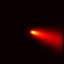
\includegraphics[width=\textwidth]{convdiff_grid.png}
        \caption{Grid of solution fields for varying $\vtheta$.}
    \end{subfigure}
    \hfill
    \begin{subfigure}[b]{0.48\textwidth}
        \centering
        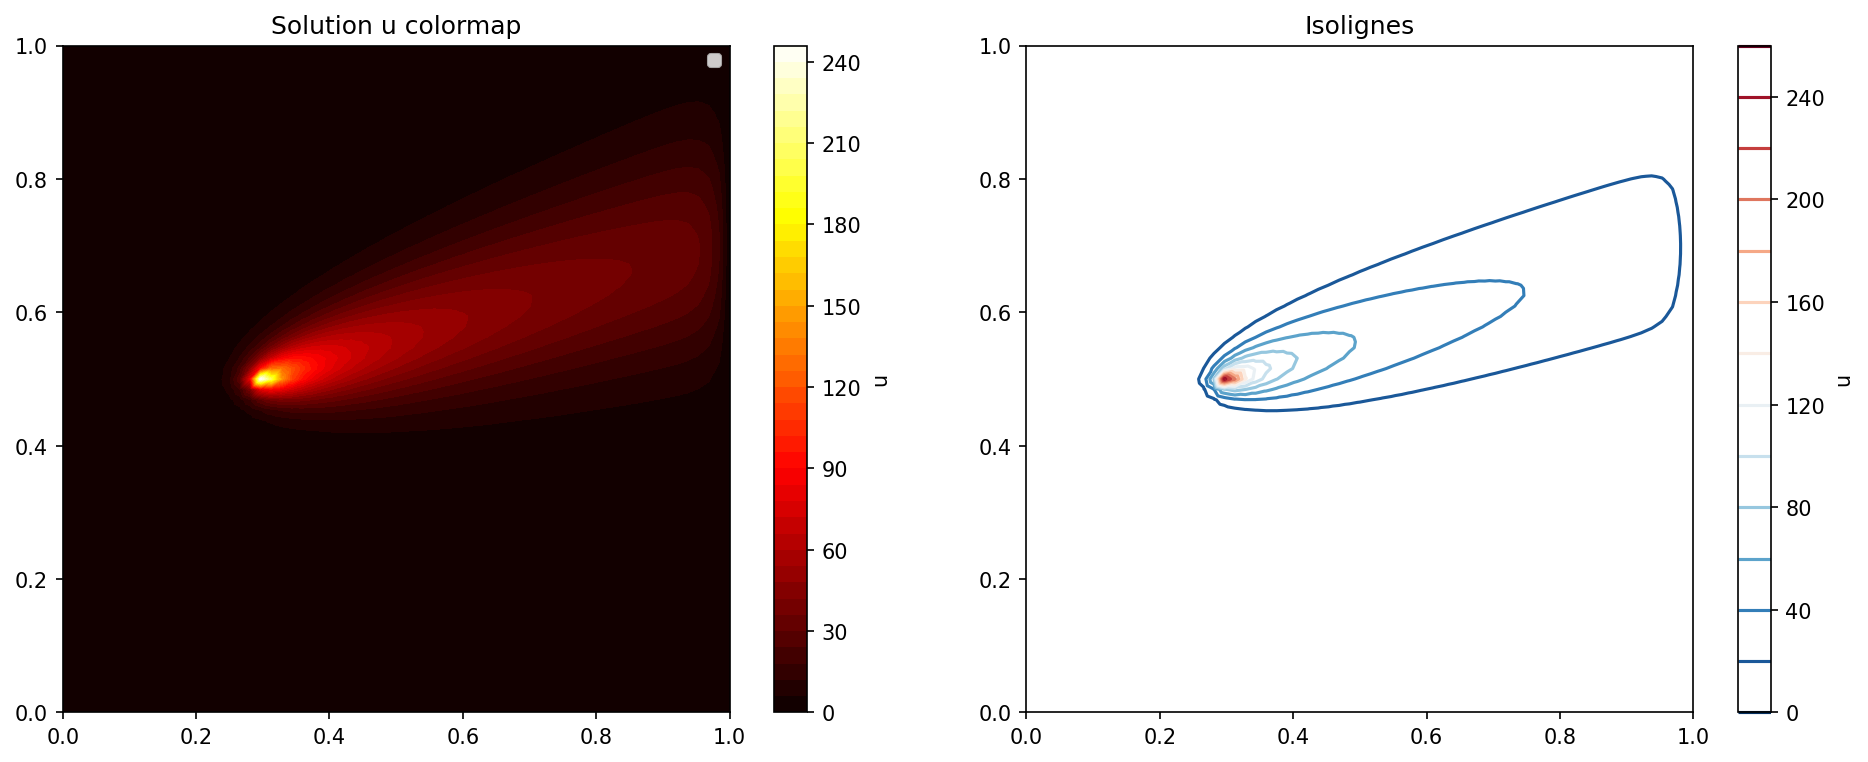
\includegraphics[width=\textwidth]{convdiff_solution.png}
        \caption{Example stationary solution $U$ on $[0,1]^2$.}
    \end{subfigure}
    \caption{Stationary convection-diffusion dataset.}
    \label{fig:convdiff}
\end{figure}

\subsection{Two-Stage Architecture}

\subsubsection{Stage 1 --- Variational Autoencoder}

A VAE compresses solution fields $U \in \R^{1 \times N \times N}$ into a low-dimensional latent code $z \in \R^{d_z}$ (default $d_z = 32$). The encoder is a four-block strided convolutional network followed by two linear heads producing the posterior mean $\mu$ and log-variance $\log \sigma^2$. The decoder maps a sampled code back through a linear projection and four ConvTranspose2d+BatchNorm+ReLU blocks to the image space.

Training minimises the negative evidence lower bound augmented with a spatial gradient penalty:
\begin{equation}
    \mathcal{L}_{\mathrm{VAE}} = \E_{q(z|U)}\bigl[\|U - \hat{U}\|^2 + \lambda_{\nabla}\|\nabla U - \nabla\hat{U}\|^2\bigr] + \beta\,\KL\bigl(q(z|U)\,\|\,\mathcal{N}(0,I)\bigr),
    \label{eq:elbo}
\end{equation}
where a \emph{free-bits} threshold per latent dimension prevents premature collapse of the KL term.

\subsubsection{Stage 2 --- Indirect Decoder \texorpdfstring{$\vtheta \to z \to U$}{theta to z to U}}

With the VAE decoder frozen, an \texttt{IndirectDecoder} network learns the regression $\vtheta \to z$ with a two-layer MLP (hidden size 128, ReLU). The predicted code is then passed through the frozen decoder. The loss is MSE on the reconstructed field plus the same spatial gradient term as in~\eqref{eq:elbo}. This two-stage strategy decouples representation learning from the parameter-to-latent regression, resulting in more stable training.

\subsection{Interactive Application}

A Streamlit application (\texttt{stationary/app.py}) wraps inference into an interactive interface: sliders expose $D$, the magnitude and angle of $\bm{b}$, and $f$, and the predicted field is optionally compared against the nearest dataset neighbour. Model and dataset loading are cached for real-time response.

\begin{figure}[ht]
    \centering
    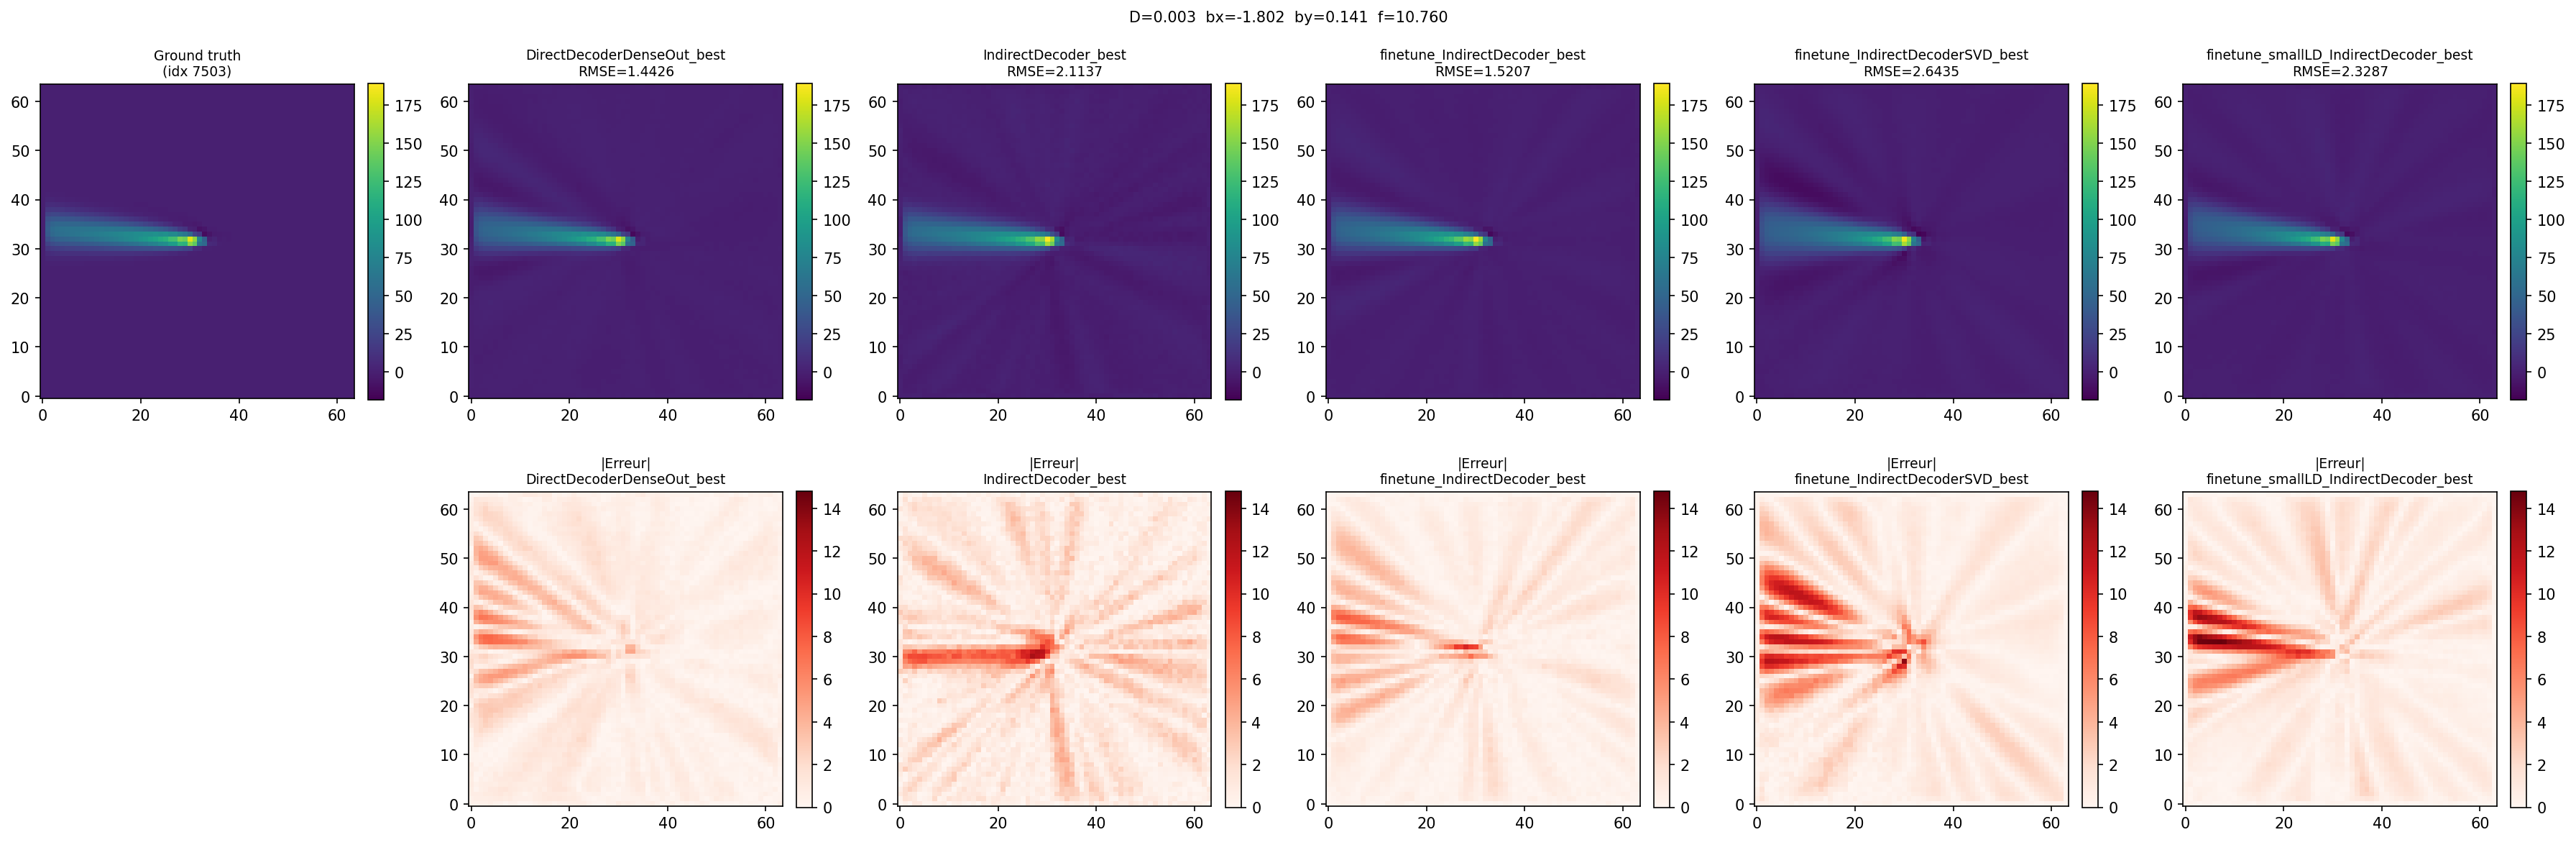
\includegraphics[width=0.72\textwidth]{demo.png}
    \caption{Streamlit interface: surrogate prediction (left) vs.\ nearest dataset sample (right).}
    \label{fig:demo}
\end{figure}

\subsection{Results}

% TODO: VAE reconstruction metrics (val/recon, val/kl) and indirect decoder
% metrics (val/loss, median relative L2 error on the test set).

% ============================================================
\section{Transient CH4 Concentration Fields}
% ============================================================

\subsection{Dataset and Problem Formulation}

\subsubsection{Dataset}

The primary dataset (\texttt{ch4\_rotated}) contains approximately 8\,100 simulations of transient CH4 concentration fields. Each simulation yields $N_t = 150$ time steps on a $200 \times 200$ spatial grid, corresponding to a raw tensor of shape $(8100, 150, 200, 200)$. Physical parameters are $\vtheta = (k, A, C)$ (reaction rate, amplitude, initial concentration) stored in \texttt{doe\_rotated.npy}. Data are accessed in memory-map mode to avoid materialising the full ${\sim}17$\,GB dataset in RAM.

\begin{figure}[ht]
    \centering
    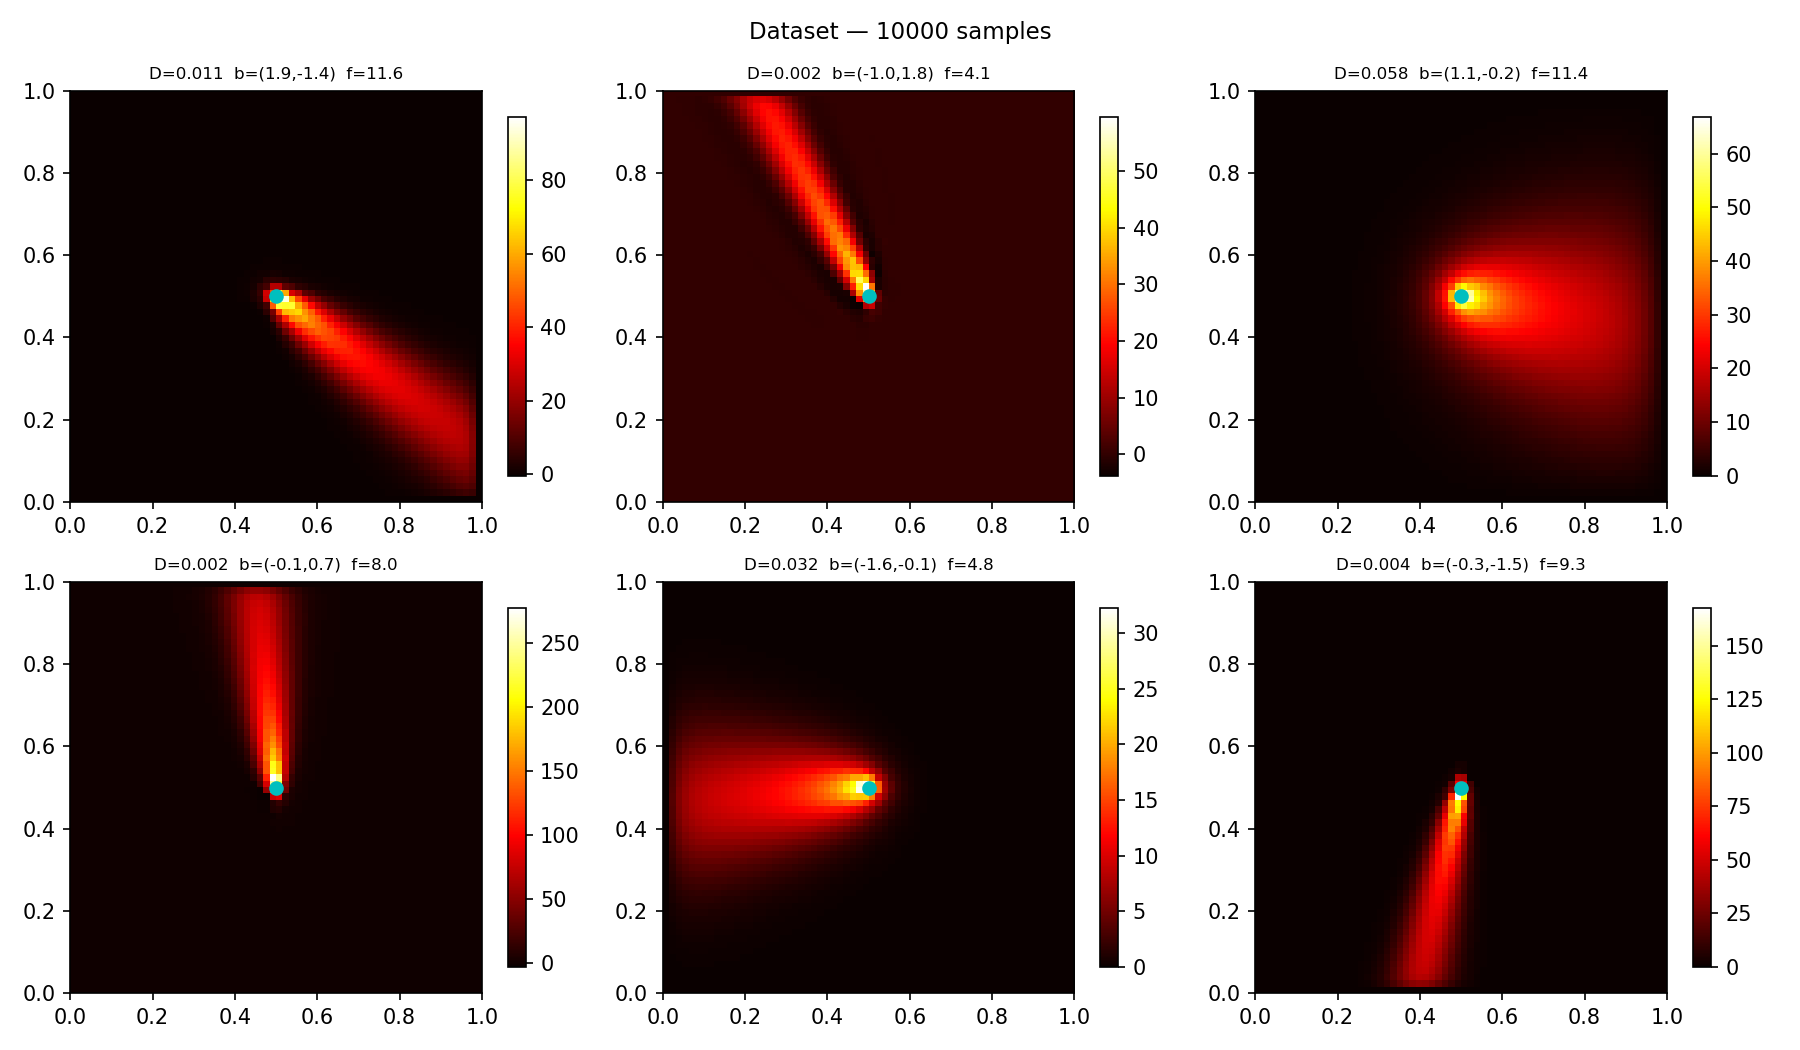
\includegraphics[width=0.82\textwidth]{dataset_preview.png}
    \caption{Dataset preview: representative CH4 concentration fields at selected time steps.}
    \label{fig:dataset}
\end{figure}

\subsubsection{Temporal Representation via the Laplace Transform}

A key modelling choice for the transient problem is to operate in the \emph{Laplace domain} rather than directly in the time domain. The numerical Laplace transform is computed along the Bromwich contour:
\begin{equation}
    \hat{U}(s_k) = \int_0^T U(t)\,e^{-s_k t}\,\mathrm{d}t
    \approx \mathrm{DFT}\bigl[U(t) \cdot w_t \cdot e^{-\gamma t}\bigr],
    \qquad s_k = \gamma + i\omega_k,
    \label{eq:laplace}
\end{equation}
where $w_t$ are trapezoidal quadrature weights and $\gamma \geq 0$ is a damping parameter. Inversion is performed by IFFT with a compensating exponential factor. By the Hermitian symmetry of real-valued signals, only the $N_{\mathrm{half}} = N_t/2 + 1$ non-redundant frequencies need to be modelled; the full spectrum is reconstructed via $\hat{U}(s_{N_t-k}) = \overline{\hat{U}(s_k)}$.

This representation decomposes the temporal dynamics into independent frequency components, enabling the construction of specialised surrogates per frequency and facilitating both latent space learning and residual correction.

\subsection{Latent Space Representation}

A central challenge in the transient setting is to find a compact, learned representation of the Laplace coefficient fields $\hat{U}(s_k) \in \C^{N \times N}$ (equivalently, the pair $(\Re(\hat{U}_k), \Im(\hat{U}_k)) \in \R^{2 \times N \times N}$). Two families of representations are explored.

\subsubsection{SVD-Based Approaches}

\paragraph{Tucker POD decomposition.}
Following the hybrid twin framework of~\cite{ammar2024hybrid}, the Tucker SVD (\texttt{utils/SVD\_Amine\_3D.py}) factorises the spatially sub-sampled training tensor $\bm{H} \in \R^{n_r \times n_s \times N_t}$ as
\begin{equation}
    H_{r,s,t} \approx \sum_{j=1}^{n_f} \alpha_j\, F_{r,j}\, G_{s,j}\, P_{t,j},
    \label{eq:tucker}
\end{equation}
with spatial basis $\bm{F}$, temporal basis $\bm{P}$, singular values $\bm{\alpha}$, and simulation-specific coefficients $\bm{G}$. Once the bases are fixed, the problem reduces to learning $\vtheta \mapsto \bm{g} \in \R^{n_f}$ with a simple MLP. This approach is extremely lightweight but fundamentally limited by the linear structure of~\eqref{eq:tucker}.

\begin{figure}[ht]
    \centering
    \begin{subfigure}[b]{0.48\textwidth}
        \centering
        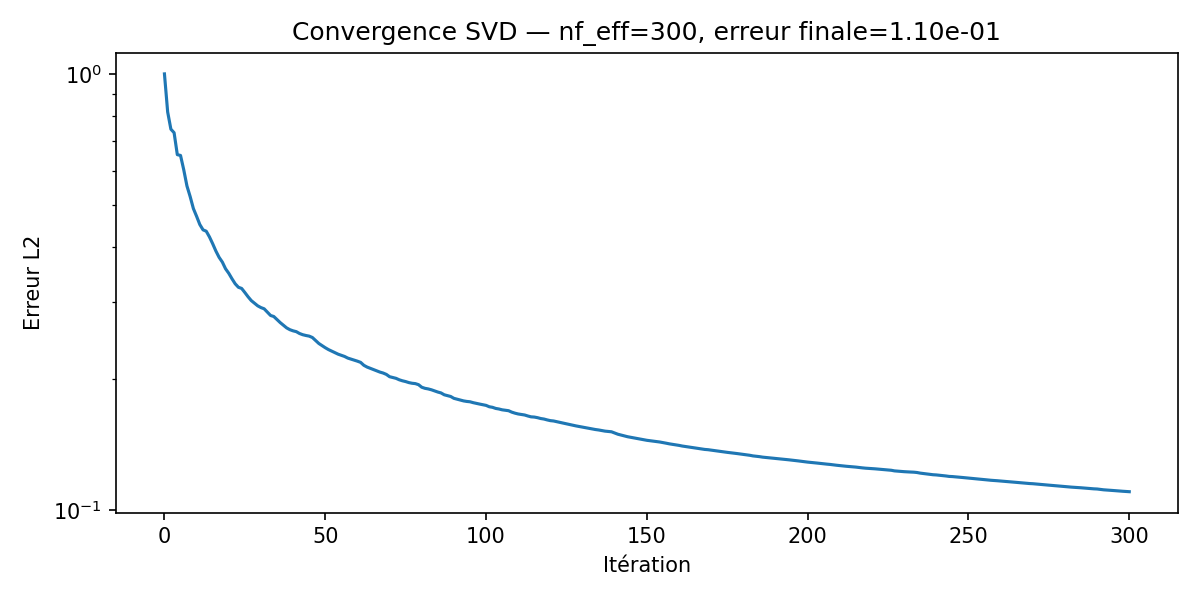
\includegraphics[width=\textwidth]{svd_convergence.png}
        \caption{Reconstruction error vs.\ number of retained modes $n_f$.}
    \end{subfigure}
    \hfill
    \begin{subfigure}[b]{0.48\textwidth}
        \centering
        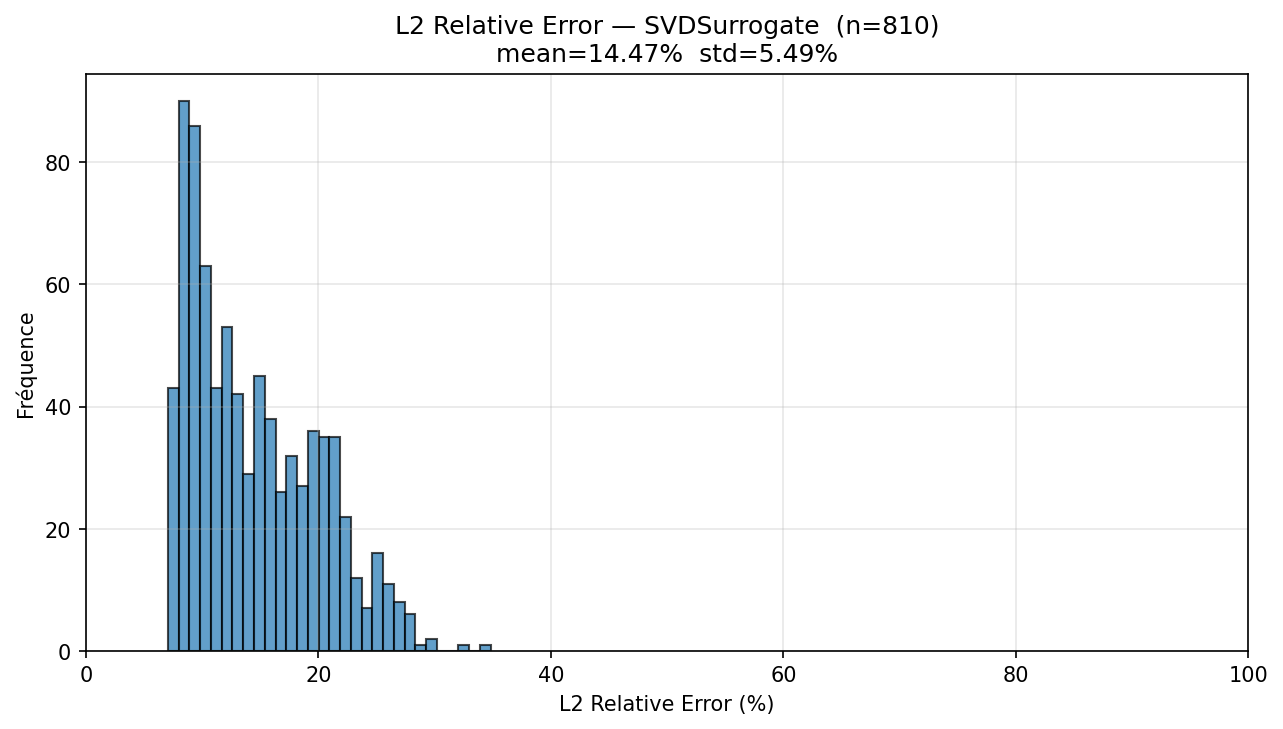
\includegraphics[width=\textwidth]{SVDSurrogate_l2rel_hist.png}
        \caption{Relative $L^2$ error on the test set (Tucker POD).}
    \end{subfigure}
    \caption{Tucker POD surrogate.}
    \label{fig:svd}
\end{figure}

\paragraph{Per-frequency SVD in the Laplace domain.}
For each Laplace frequency $k$, a truncated SVD is computed on the matrix of training coefficients (real and imaginary parts independently):
\[
    \Re(\hat{\bm{U}}_k) \approx \bm{c}^{(k,r)} \bigl(\bm{V}^{(k,r)}\bigr)^\top, \quad
    \Im(\hat{\bm{U}}_k) \approx \bm{c}^{(k,i)} \bigl(\bm{V}^{(k,i)}\bigr)^\top,
\]
where $\bm{V} \in \R^{N^2 \times k_{\mathrm{svd}}}$ and $\bm{c} \in \R^{k_{\mathrm{svd}}}$ are the leading right singular vectors and associated coefficients respectively. A lightweight three-layer MLP per frequency then predicts the normalised coefficients $\hat{\bm{c}}$. This approach, implemented as \texttt{LaplaceSVDModel}, combines the Laplace decomposition with a linear spatial basis, enabling frequency-specific compression.

\begin{figure}[ht]
    \centering
    \begin{subfigure}[b]{0.48\textwidth}
        \centering
        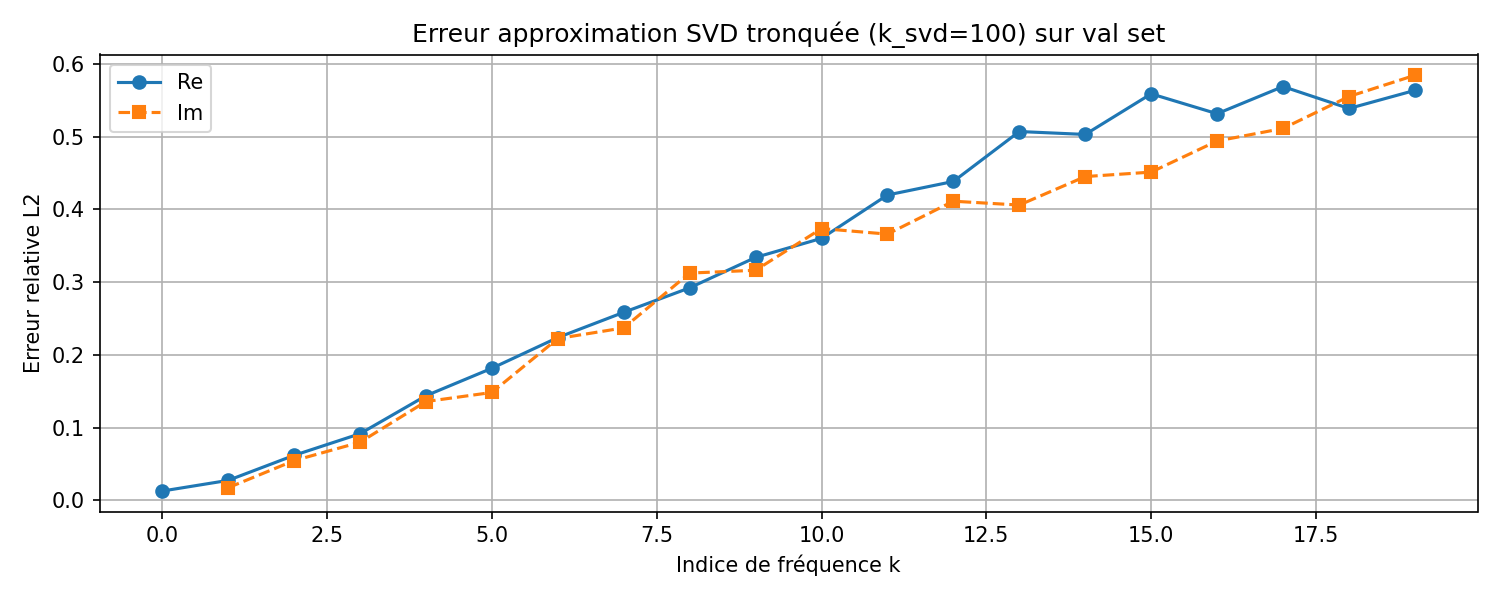
\includegraphics[width=\textwidth]{LaplaceSVDModel_svd_error_ksvd100.png}
        \caption{SVD reconstruction error vs.\ number of components ($k_{\mathrm{svd}} = 100$).}
    \end{subfigure}
    \hfill
    \begin{subfigure}[b]{0.48\textwidth}
        \centering
        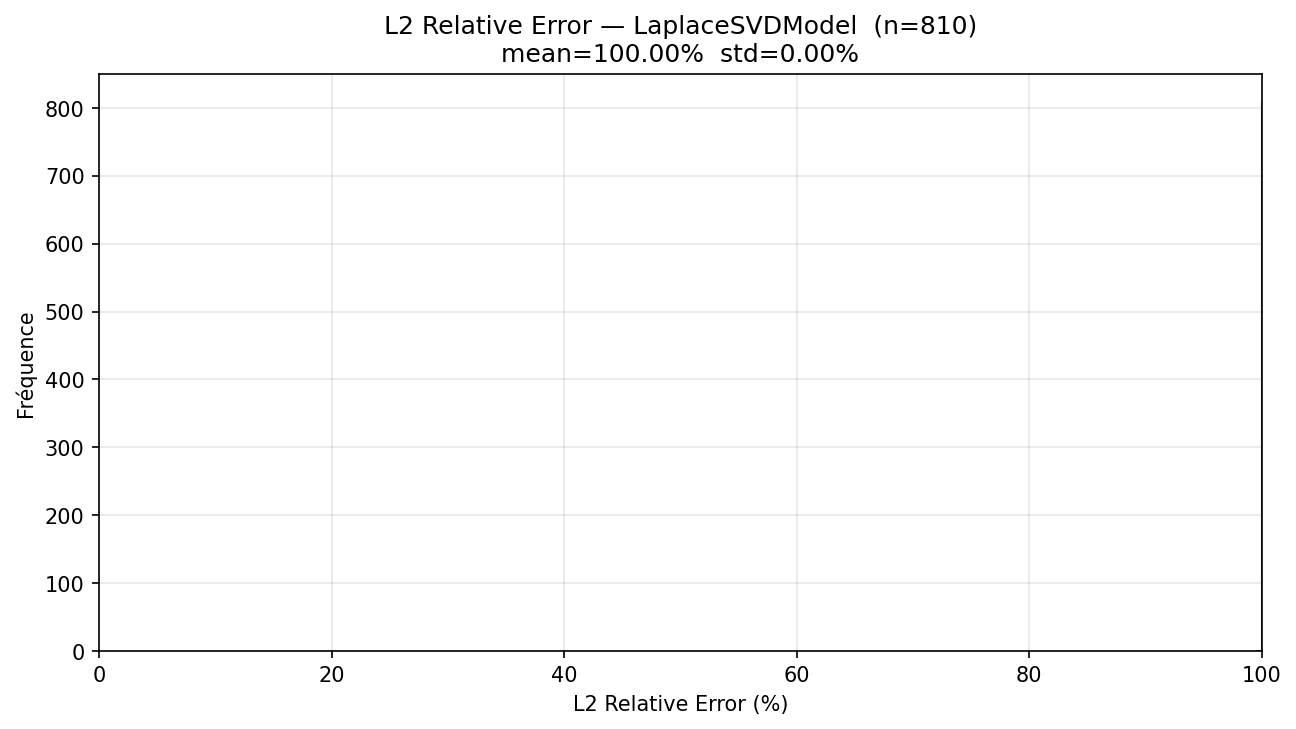
\includegraphics[width=\textwidth]{LaplaceSVDModel_l2rel_hist.png}
        \caption{Relative $L^2$ error on the test set (Laplace SVD).}
    \end{subfigure}
    \caption{SVD surrogate in the Laplace domain.}
    \label{fig:lapsvd}
\end{figure}

\paragraph{Limitations of SVD-based representations.}
Both SVD approaches impose a \emph{linear} structure on the latent space: the field $\hat{U}_k$ is constrained to lie in a fixed linear subspace spanned by pre-computed basis vectors. While this is computationally simple and theoretically well-founded for low-rank fields, it becomes a bottleneck when the physical fields exhibit complex, non-linear variation across the parameter space. In particular, the spatial structures of $\hat{U}_k$ can vary non-linearly with $\vtheta$, making a fixed linear basis suboptimal.

\subsubsection{Autoencoder-Based Latent Space}

To overcome the linearity constraint, we learn a non-linear latent space via a frequency-conditioned autoencoder (\texttt{LaplaceAE}, \texttt{models/laplace\_ae\_surrogate.py}).

\paragraph{Sinusoidal frequency conditioning.}
Since a single autoencoder must handle Laplace fields at all frequencies simultaneously, it is conditioned on the normalised frequency ratio $f = k/N_{\mathrm{half}} \in [0,1]$. A NeRF-style sinusoidal positional encoding provides a dense, multi-resolution representation of this scalar:
\begin{equation}
    \bm{e}(f) = \mathrm{MLP}\Bigl(\bigl[\sin(2^i\pi f),\; \cos(2^i\pi f)\bigr]_{i=0}^{L-1}\Bigr) \in \R^{64},
    \label{eq:posenc}
\end{equation}
with $L = 8$ frequency levels. This encoding allows the network to discriminate between neighbouring Laplace frequencies while capturing coarse spectral structure through the lower-frequency components.

\paragraph{Architecture.}
The FiLM (Feature-wise Linear Modulation) mechanism \cite{perez2018film} injects the frequency embedding at each network layer by computing affine modulation parameters $(\gamma_\ell, \beta_\ell)$ from $\bm{e}(f)$:
\begin{equation}
    \bm{x} \leftarrow \bm{x} \odot (1 + \gamma_\ell) + \beta_\ell.
    \label{eq:film}
\end{equation}
The encoder (\texttt{LaplaceEncoder}) applies three strided Conv2d blocks ($2 \to 16 \to 32 \to 64$ channels, stride 2), each followed by FiLM conditioning, then maps the spatial features to $z \in \R^{d_z}$ via two linear layers. The scaling parameters $\gamma_\ell$ are passed through $\tanh$ to avoid numerical instability in half-precision training. The decoder (\texttt{LaplaceDecoder}) reverses this with three ConvTranspose2d+BatchNorm+ReLU blocks, FiLM-modulated at each level, followed by two independent refinement branches (one for $\Re$, one for $\Im$) that produce the final two-channel output.

The training objective combines reconstruction MSE and a ridge regularisation on the decoder outputs:
\begin{equation}
    \mathcal{L}_{\mathrm{AE}} = \|\hat{U} - U\|^2 + \beta\,\|\hat{U}\|^2.
    \label{eq:aeloss}
\end{equation}
The training dataset is flattened over the (simulation, frequency) dimensions and reshuffled between epochs to prevent frequency-specific overfitting.

\paragraph{Advantage over SVD.}
The autoencoder latent space is non-linear, adaptive, and jointly trained across all frequencies. The shared encoder and decoder weights are specialised to each frequency only through the lightweight FiLM modulation, enabling efficient parameter sharing without sacrificing frequency-specific expressiveness. Empirically, this leads to lower reconstruction error than SVD at comparable latent dimensionality $d_z$.

\subsection{Surrogate and Fine-Tuning}

\subsubsection{Per-Frequency Surrogate \texorpdfstring{$\vtheta \to z$}{theta to z}}

With the \texttt{LaplaceAE} trained and its decoder frozen, we train one lightweight MLP per Laplace frequency to learn the regression $\vtheta \to z_k$ (\texttt{LaplaceLatentSurrogate}). Each surrogate consists of a four-layer MLP (\texttt{proj}) with LayerNorm after each linear transformation:
\begin{equation}
    \vtheta_{\mathrm{norm}} \;\xrightarrow{d_h/2}\; \xrightarrow{d_h}\; \xrightarrow{d_h}\; d_z,
    \label{eq:proj}
\end{equation}
where $d_h = 256$ is the hidden width. The shared decoder is injected by reference (not registered as a submodule), avoiding any weight duplication in GPU memory.

The assembled \texttt{LaplaceLatentModel} contains $N_{\mathrm{half}}$ such surrogates together with a single frozen \texttt{shared\_decoder}. At inference, all projections $\{\vtheta \to z_k\}$ are computed in parallel, then a single batched decoder call produces the entire Laplace spectrum:
\begin{equation}
    \{z_k\}_{k=0}^{N_{\mathrm{half}}-1} \;\xrightarrow{\text{batched}}\; \text{shared\_decoder} \;\to\; \{\hat{U}_k\}_k.
\end{equation}
The time series is recovered by Hermitian symmetry completion followed by IFFT inversion of the Bromwich integral~\eqref{eq:laplace}.

\subsubsection{End-to-End Fine-Tuning}

After independent per-frequency training of the \texttt{proj} networks, the shared decoder is unfrozen and the complete model is fine-tuned end-to-end (\texttt{transient/finetune\_decoder\_laplace.py}). Differential learning rates are applied: the surrogate MLPs are updated with a larger step size $\eta_{\mathrm{surr}} = 5 \times 10^{-5}$, while the decoder uses a smaller rate $\eta_{\mathrm{dec}} = 10^{-5}$, preserving the learned spectral decoder structure while allowing it to adapt to the surrogate outputs. The fine-tuning dataset is reorganised in frequency-first order so that each mini-batch covers all training simulations for a single frequency, enabling a single batched decoder call per gradient step and substantially reducing wall-clock time.

\begin{figure}[ht]
    \centering
    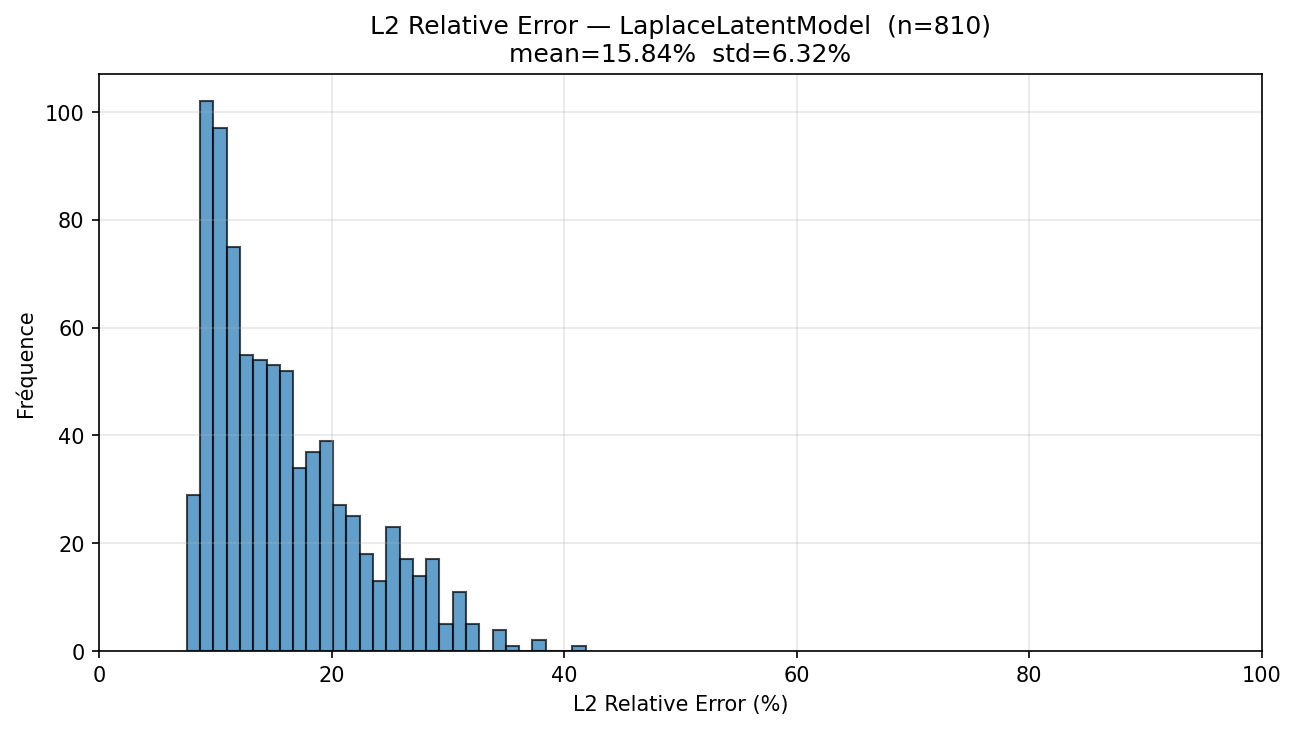
\includegraphics[width=0.55\textwidth]{LaplaceLatentModel_l2rel_hist.png}
    \caption{Relative $L^2$ error on the test set after end-to-end fine-tuning (latent Laplace surrogate).}
    \label{fig:laplacelatent}
\end{figure}

\subsubsection{Results}

% TODO: median relative L2 error before and after fine-tuning; comparison with Tucker POD and Laplace SVD.

% ============================================================
\subsection{Post-Processing and Results}
% ============================================================

\subsubsection{Residual Correction}

Laplace-based surrogates can exhibit oscillatory artefacts—particularly near sharp transitions and in high-gradient regions—due to the finite number of retained spectral frequencies and residual surrogate approximation error. Rather than retraining the surrogate, a lightweight residual corrector is applied \emph{post hoc} frame by frame, learning only the systematic error pattern.

The \texttt{CorrectionAE} (\texttt{models/correction\_ae.py}) is a three-level UNet. Given a predicted frame $U_{\mathrm{pred}} \in \R^{N \times N}$, it is first normalised per-sample: $\tilde{U} = (U_{\mathrm{pred}} - \mu)/\sigma$. The encoder applies three double-convolution blocks (Conv2d $3\times3$ + ReLU, $\times2$) with MaxPool2d downsampling, with channel progression $1 \to c \to 2c \to 4c$ ($c = 16$). A bottleneck at resolution $N/8$ uses $8c$ channels. The decoder reverses the encoder with ConvTranspose2d upsampling, concatenating skip connections at each level. The output $1\times1$ convolution is \textbf{zero-initialised}, so the model starts from the identity (zero residual correction) and learns corrections gradually:
\begin{equation}
    U_{\mathrm{corr}} = U_{\mathrm{pred}} + \sigma \cdot r\!\left(\tilde{U}\right),
    \label{eq:correction}
\end{equation}
where $r(\cdot)$ denotes the UNet output. With base channel width $c = 16$, the model has approximately 481\,000 parameters.

\subsubsection{Training the Corrector}

To avoid repeated expensive calls to the base surrogate, all $(U_{\mathrm{pred}}, U_{\mathrm{true}})$ pairs are pre-computed and stored as memory-mapped arrays of shape $(n_s, k_t, N, N)$ on disk ($k_t = 20$ randomly sampled frames per simulation). The surrogate is then freed from GPU memory before corrector training begins.

The training objective is an MSE on the normalised residual augmented by a spatial gradient matching term:
\begin{equation}
    \mathcal{L}_{\mathrm{corr}} = \left\|\frac{r_{\mathrm{pred}} - r_{\mathrm{true}}}{\sigma_r}\right\|^2 + \lambda_{\nabla}\left\|\frac{\nabla r_{\mathrm{pred}} - \nabla r_{\mathrm{true}}}{\sigma_r}\right\|^2,
    \label{eq:corrloss}
\end{equation}
where $r_{\mathrm{pred}} = U_{\mathrm{corr}} - U_{\mathrm{pred}}$, $r_{\mathrm{true}} = U_{\mathrm{true}} - U_{\mathrm{pred}}$, $\sigma_r = \sigma(r_{\mathrm{true}})$, and $\lambda_{\nabla} = 10$.

\subsubsection{Full Pipeline}

The \texttt{CorrectedPipeline} class inherits from \texttt{LaplaceLatentModel} and overrides the generation step: after Laplace inversion, all frames pass through the correction UNet in chunks of 64 to manage GPU memory. Surrogate modules are shared by reference with no weight duplication.

\subsubsection{Results and Comparison}

\begin{figure}[ht]
    \centering
    \begin{subfigure}[b]{0.48\textwidth}
        \centering
        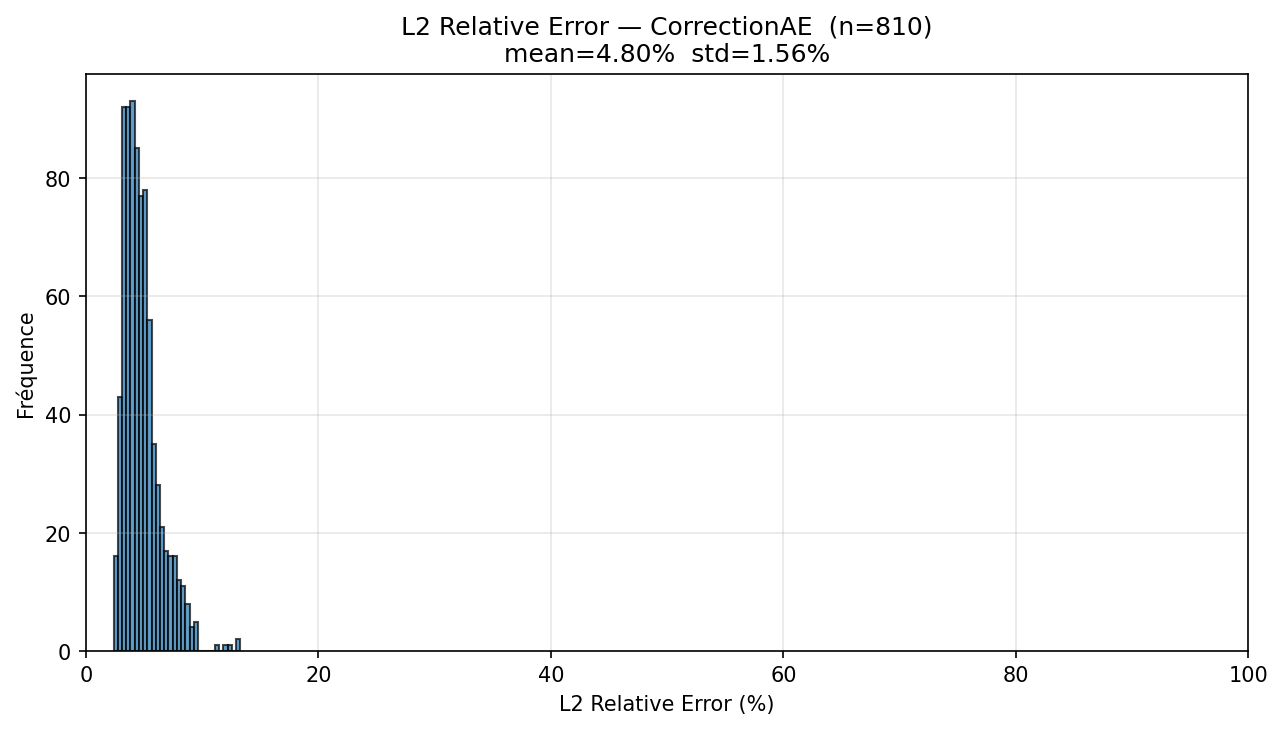
\includegraphics[width=\textwidth]{CorrectionAE_l2rel_hist.png}
        \caption{Relative $L^2$ error distribution after residual correction.}
    \end{subfigure}
    \hfill
    \begin{subfigure}[b]{0.48\textwidth}
        \centering
        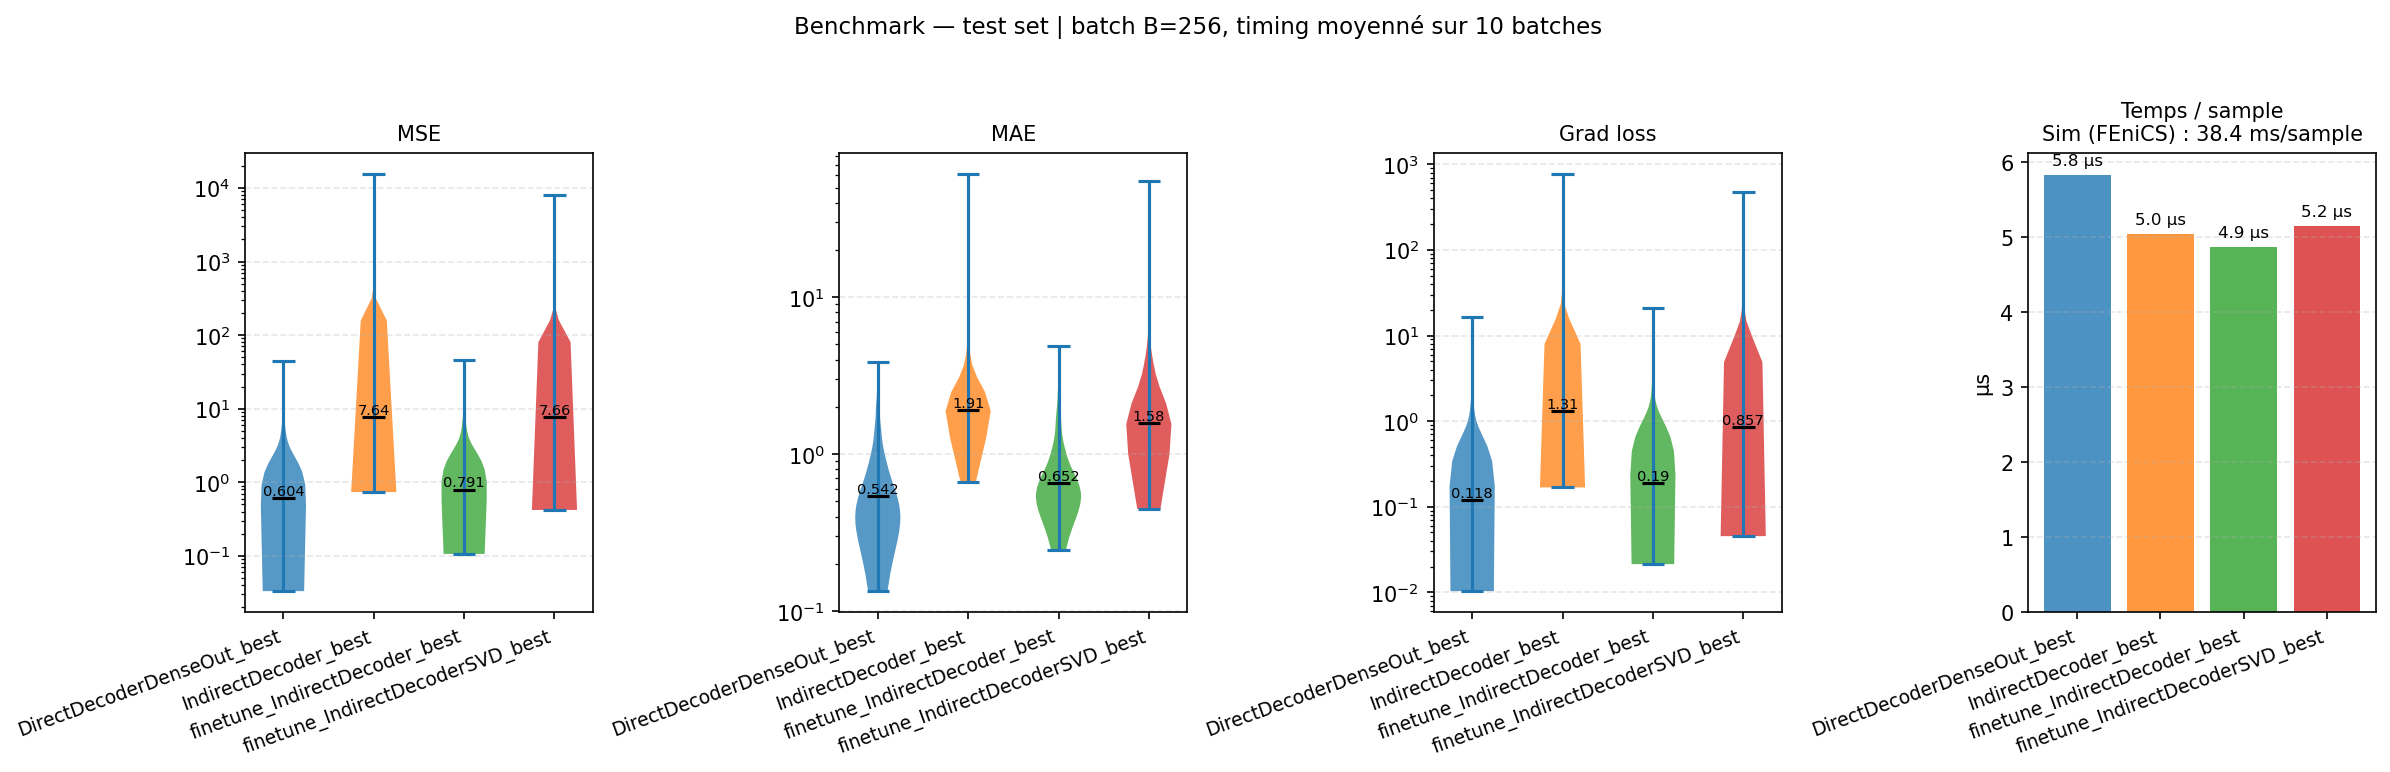
\includegraphics[width=\textwidth]{benchmark.png}
        \caption{Pipeline comparison on the test set.}
    \end{subfigure}
    \caption{Residual correction post-processor and overall comparison.}
    \label{fig:correction}
\end{figure}

\begin{table}[ht]
    \centering
    \begin{tabular}{lccc}
        \toprule
        \textbf{Method} & \textbf{Representation} & \textbf{Parameters} & \textbf{Median $L^2_{\mathrm{rel}}$ (\%)} \\
        \midrule
        Tucker POD           & POD coefficients $\bm{g}$       & ${\sim}$1\,M          & --- \\
        Laplace SVD          & SVD coefficients per frequency   & ---                   & --- \\
        Latent Laplace       & Shared autoencoder latent code   & ---                   & --- \\
        Latent Laplace + AEC & + UNet residual correction       & $+481$k               & --- \\
        \bottomrule
    \end{tabular}
    \caption{Comparison of transient surrogates on the test set. Numeric entries to be filled.}
    \label{tab:comparison}
\end{table}

% TODO: fill in parameter counts, median L2rel for each method, inference time if available.
% Provide qualitative frame examples before/after correction.

% ============================================================
\section{Conclusion}
% ============================================================

This work presents a complete hierarchy of neural surrogate architectures for PDE emulation, progressing from classical POD regression to sophisticated non-linear latent-space generative models. The preliminary study on the stationary convection-diffusion problem demonstrates the effectiveness of the VAE two-stage paradigm and validates the infrastructure for data generation, normalisation, and inference.

For the more challenging transient problem, the Tucker POD and SVD-in-Laplace approaches establish competitive baselines under a linear compression assumption. The frequency-conditioned \texttt{LaplaceAE} overcomes this limitation by learning an adaptive, non-linear latent space shared across all spectral frequencies, achieving better reconstruction at comparable latent dimensionality. The subsequent per-frequency MLP surrogates, refined through end-to-end fine-tuning, produce accurate predictions of the full spatio-temporal field.

Finally, the lightweight UNet residual corrector demonstrates that a post-processing step of modest capacity (481k parameters) can substantially reduce oscillatory artefacts without retraining the base surrogate. The resulting \texttt{CorrectedPipeline} combines the best of both worlds: a structured spectral representation with non-linear latent space learning and a data-driven correction stage.

Future directions include incorporating physics-informed constraints into the latent space, extending the framework to varying geometries, and applying the residual corrector to other reduced-order surrogate families beyond the Laplace representation.

\begin{thebibliography}{9}
    \bibitem{perez2018film}
    E.~Perez, F.~Strub, H.~de Vries, V.~Dumoulin, and A.~Courville.
    \emph{FiLM: Visual Reasoning with a General Conditioning Layer}.
    In \emph{Proceedings of the AAAI Conference on Artificial Intelligence}, 2018.

    \bibitem{ammar2024hybrid}
    A.~Ammar, M.~Ben~Saada, E.~Cueto, and F.~Chinesta.
    Casting hybrid twin: physics-based reduced order models enriched with
    data-driven models enabling the highest accuracy in real-time.
    \emph{International Journal of Material Forming}, 17(16), 2024.
    \texttt{doi:10.1007/s12289-024-01812-4}, hal-05056779.
\end{thebibliography}

\end{document}
